\chapter{Hierarchical Fault Dictionary}
\label{chap:dict}

The goal of on-chip test and diagnosis is to provide robustness against early-life and wear-out failures, through periodic self-test and self-diagnosis.
%
Once a test failure is detected, the failure must be localized (diagnosed) to determine which module of the tested core/uncore is defective.
%
A fault dictionary is one method of performing fault diagnosis, and the dictionary is a pre-computed table of expected circuit behavior in the presence of each modeled fault.
%
For testing a complex modern System on Chip (SoC), a high-quality set of two-vector tests plus a fault dictionary are created for each unique core or uncore in the SoC.
%
During normal operation in the field, the test and diagnosis controller selects a core/uncore for test, isolates it from the rest of the SoC, applies the corresponding test set while recording the test responses, and upon detecting failure, finally uses the fault dictionary and the recorded test responses for localization via the on-chip diagnosis hardware.

As previously mentioned, the few economically-feasible recovery options available at runtime (namely to repair, replace, or avoid a defect) are too expensive to be implemented at a fine level of granularity.
%
That is, it is not viable to repair a single transistor, or replace a particular flip-flop.
%
These recovery actions are only practical for larger modules at a higher level of the design hierarchy.
%
While the goal of conventional fault diagnosis is to localize the failure to a specific modeled fault, on-chip diagnosis only needs to localize a failure to the level of repair, replacement, or avoidance, also known as the level of \textit{recovery}.
%
This relaxation of diagnosis precision enables the removal of faults from the dictionary that are not necessary for performing recovery-level diagnosis.

A fault dictionary is a tabulation of expected circuit responses (or some subset thereof) for each modeled fault considered, for each test (or test pair) in the test set.
%
It is convenient to view a fault dictionary as a table of values (fault simulation responses) with one row for each fault and one column for each test pair.
%
A fault dictionary that contains the full response for each fault/test pair is a \textit{full-response dictionary}.
%
Traditional diagnosis searches the rows of the fault dictionary to find the fault that matches (or is the most similar to) the observed behavior of a faulty circuit.
%
For the TRAX fault model, where an exact match between a modeled fault and defective circuit is not expected, a more complex diagnosis process is required, as detailed in Chapter~\ref{chap:diag}.
%
The rest of this chapter details the creation of a new fault dictionary with increased compaction, owing to the reduced recovery-level localization requirements of on-chip diagnosis.

A full-response fault dictionary requires a large amount of storage, equal to the product of the number of faults, the number of tests, and the number of circuit primary outputs, which can be quite large for modern designs.
%
For example, the circuit L2B~\cite{sun11} contains just over 12,000 gates and uses 90 test vector pairs for test and diagnosis.
%
The full-response fault dictionary for L2B requires over 600 megabytes of storage, which is impractical for on-chip diagnosis for this relatively small circuit.
%
To reduce the size required to store a fault dictionary, a variety of compaction schemes~\cite{arslan02, bernardi06, boppana94, chakravarty99, boppana96, chess99, hong07, pomeranz92} have been developed for reducing the size of a fault dictionary, each exhibiting their own trade-off between diagnostic resolution and dictionary size/complexity.
%
Existing techniques are effective but do not enable a sufficient level of compaction when applied to modern designs~\cite{ryan93, boppana94}.
%
One straightforward compaction technique is only to include faults relating to the targeted defect model (i.e., NBTI and ELF).
%
To this end, the TRAX fault dictionary explored here only includes faults located at standard-cell outputs since NBTI and ELF affect the delay of standard cells.
%
Elimination of the remaining faults (i.e., faults located at primary inputs or fanout branches) reduces dictionary size through the removal of dictionary rows.

Given that system resources for test and diagnosis must be limited, it is not feasible to store the entire simulation response of every fault.
%
Instead, a single bit per test is stored to indicate pass/fail status of the corresponding simulation response, resulting in a pass/fail dictionary.
%
A pass/fail dictionary is a well-known technique for significantly reducing the size of a fault dictionary at the expense of diagnostic resolution~\cite{pomeranz92}.
%
Resolution degradation, however, is minimal since the level of precision required is limited to the level of recovery.
%
Specifically, for all benchmark circuits analyzed, the resolution loss averaged less than 0.023\%, where resolution is equated to the number of distinguished fault pairs divided by the total number of fault pairs.

\section{Module-Level Hierarchy}
\label{sec:dict_mod_level_hier}

For on-chip test and diagnosis, the tested core or uncore~\cite{li08, inoue08} is assumed to be partitioned into a set of interconnected modules, each of which can be independently repaired, replaced, or avoided if found to be faulty.
%
Figure~\ref{fig:dict_core_uncore_modules_faults} illustrates an example system-on-chip (SoC) that contains three cores/uncores which themselves are composed of multiple modules that include TRAX faults shown as circles within each module.
%
The modules within each core/uncore are assumed to be at the recovery-level.
%
In other words, these modules are at the finest level of granularity for which recovery can be cost-effectively deployed.
%
Put another way, it would be ideal if the actual transistor responsible for slowdown could be both identified and handled via repair, replacement, or avoidance.
%
Achieving robustness however at this very fine level of granularity is much too costly.
%
So instead, the level of recovery is defined to be the set of sub-circuits (i.e., modules) within a core or uncore that can be effectively handled by repair, replacement, or avoidance.
%
We make no assumptions however how small or large these modules should be since there are challenging tradeoffs involving performance, power, and robustness.
%
Regardless of how these modules are defined, the approach for on-chip diagnosis described here remains applicable, albeit with an associated level of efficiency and effectiveness that is dependent on core/uncore partitioning into modules.
%
Finally, it is also important to point out that the core/uncore is the smallest testable entity.
%
That is, we assume it is not cost-effective to test each module within a core/uncore separately from all other modules.
%
If this were not true, then diagnosis would be unnecessary since test failure alone would identify the culprit module.

%\vskip 0.5em%
\begin{figure}[hbtp]
\centering
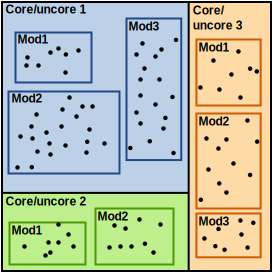
\includegraphics[width=0.4\columnwidth]{fig_core_uncore_modules_faults}
\caption{Hierarchical view of a system-on-chip (SoC) that contains multiple cores and uncores, each of which contain multiple modules.
%
Within each module are a number of faults.}
\label{fig:dict_core_uncore_modules_faults}
\end{figure}
%\vskip 0.5em%

One example of sub-module repair is presented in~\cite{hsiung15}, where a multi-layered approach is used to provide defect-tolerance and improve yield.
%
The layers analyzed include circuit-, microarchitecture-, and ISA-layers.
%
At each layer, workload analysis is used to determine if there are any sub-modules that occupy a disproportional amount of the workload or circuit area, potentially leading to a more fine-grained repair option.
%
As an example, for the ALU analyzed at the microarchitecture-layer, the coarse approach would be to disable an entire ALU found to be faulty.
%
Through workload and circuit analysis, the multiplier sub-module is determined to occupy a large percentage of the ALU area, and that a majority of multiplication operations performed only require accuracy in the lower $N$ bits of the product.
%
This permits a more fine-grained repair approach where such limited-output-size multiply operands can continue to use such a partially-damaged ALU.
%
As another example, many circuits contain arrays of identical structure, such as the full-adder blocks of a multi-bit adder module.
%
The approach presened in~\cite{hsiung15} recognizes that if the repeated circuit structures are not all free from defects, a small amount of additional data steering logic can be used to iteratively perform a calculation with partially-faulty hardware.
%
While this paper does not address the diagnosis process necessary to determine which module or sub-modules are faulty, it does provide an example of circuit repair performed within a single block of combinational logic, much like the approach assumed in this dissertation.

Because of the recovery level, on-chip diagnosis is significantly eased as compared to conventional approaches since precision can be relaxed to the module-level of localization.
%
Existing dictionary compaction techniques have not considered this relaxation in diagnosis precision and are therefore not directly applicable to the on-chip diagnosis task formulated here.
%
In other words, diagnosing to the recovery level means that circuit-level resolution (e.g., signal line, standard cell, or layout) can be replaced with module-level resolution to achieve a smaller dictionary size.
%
In addition, this means that only certain inter-module fault pairs have to be distinguished within the fault dictionary (i.e., have dictionary rows where at least one entry is different).


\section{Fault Equivalence and Subsumption}
\label{sec:dict_fault_equ_sub}

For intra-module faults that are test-set equivalent (identical simulation responses for all tests), all but one can be eliminated since distinguishing them using advanced diagnosis techniques (e.g.,~\cite{desineni05}) is now unnecessary.
%
Other intra-module faults can also be eliminated based on subsumption.
%
Subsumption is similar to dominance but is subtly different due to the use of the \textit{X} value and the opposite way it is exploited to reduce the fault universe.
%
A fault $c$ is said to subsume another fault $d$, if $c$ and $d$ are not test-set equivalent and the erroneous test response of $c$ subsumes the erroneous response of $d$.
%
In other words, fault $c$ subsumes fault $d$ if $c$ produces an \textit{X} value for all the same tests and outputs as fault $d$, and their fault-simulation responses are not identical.
%
A subsumed fault (e.g., fault $d$) can be eliminated since, if it exists, it will produce a response that can also be produced by fault $c$\footnote{It should be noted that fault subsumption is only valid for a fault model such as TRAX since conventional fault models have only a single simulation response.
%
TRAX faults, on the other hand, have a set of possible responses given that the observed X values all do not have to correspond to errors.}.
%
Again, since faults $c$ and $d$ are in the same module, there is no need to distinguish them.
%
Note that the subsuming fault (e.g., fault $c$) cannot be eliminated since it could produce a response that is not captured by another fault in the module, thus making it possible that it would not be distinguished from some other fault outside the module if it were removed.

Using subsumption to eliminate faults is not the same as dominance-based fault collapsing.
%
First, in dominance collapsing, the dominating fault (e.g., fault $c$) is the one collapsed.
%
Second, and more importantly, dominance-collapsed faults cannot be altogether eliminated in an application such as ATPG since they must still be explicitly considered if a test cannot be found for any of its dominated faults.

%\vskip 0.5em%
\begin{table}[hbtp]
\centering
\begin{tabular*}{0.9\columnwidth}{@{\extracolsep{\fill}}cccccccl}
\toprule
Fault&Module&$T_1$&$T_2$&$T_3$&$T_4$&$T_5$&\\
\midrule
$F_1$&$M_1$&P&F&F&P&F&\\
$F_2$&$M_1$&P&F&F&P&F&Eliminated (EQU)\\
$F_3$&$M_1$&P&F&P&P&P&Eliminated (SUB)\\
$F_4$&$M_1$&F&F&P&P&F&\\
\midrule
$F_5$&$M_2$&F&F&P&P&F&\\
$F_6$&$M_2$&P&P&F&F&P&\\
\bottomrule
\end{tabular*}
\caption{TRAX fault dictionary data illustrates dictionary compaction, using equivalence and subsumption relationships to eliminate two intra-module faults.
%
Specifically, $F_2$ is eliminated due to equivalence with $F_1$, and $F_3$ is eliminated because it is subsumed by both $F_1$ and $F_4$.}
\label{table:dict_fault_resp}
\end{table}
%\vskip 0.2em%

In the context of on-chip diagnosis, where test and diagnosis resources are limited, it is only feasible to store the test responses as a single pass/fail bit.
%
Instead of analyzing full-responses, fault elimination through equivalence and subsumption is performed using the pass/fail response from each test.
%
An example of this process is shown in Table~\ref{table:dict_fault_resp}.
%
Specifically, fault $F_2$ is eliminated via equivalence with $F_1$, and $F_3$ is eliminated because it is subsumed by both $F_1$ and $F_4$.
%
These two techniques for fault reduction are only applied to faults belonging to the same module because recovery-level diagnosis does not require distinguishing intra-module faults.
%
Applying these dictionary compaction techniques produces a \textit{collapsed pass/fail hierarchical dictionary}, which is used in the diagnosis experiments presented later.
%
For the L2B fault dictionary mentioned before, the full-response dictionary of over 600 megabytes is compacted to less than 32 kilobytes for the collapsed pass/fail dictionary.


\section{Experiments}
\label{sec:dict_exp}
A variety of experiments are performed to evaluate a collapsed pass/fail hierarchical dictionary based on the TRAX fault model.
%
Specifically, hierarchical fault dictionaries are built for 22 benchmark circuits, for the TF, TRAX, and UTF fault models, presented in Section~\ref{sec:dict_exp_size_res}.
%
The sensitivity of diagnosis results to the level of circuit partitioning is analyzed in Section~\ref{sec:dict_exp_partitioning}.


\subsection{Dictionary Size and Resolution}
\label{sec:dict_exp_size_res}

As previously mentioned, measuring dictionary size reduction due to fault elimination requires access to designs that exhibit module-level hierarchy.
%
The hierarchical versions of the ISCAS85 benchmark circuits~\cite{brglez85} (modified by~\cite{hansen99}) serve this purpose since many of the benchmarks have been reverse engineered to at least two levels of hierarchy.
%
Additionally, seven circuits are taken from the ITC99 benchmark set~\cite{corno99}, two circuits are taken from the OpenSPARC T2 design~\cite{sun11}, and five circuits are taken from the EPFL Combinational Benchmarks suite~\cite{epfl}.
%
Unlike the ISCAS85 benchmark circuits, these additional circuits are not pre-partitioned into module-level hierarchy and are instead partitioned into ten modules each using graph clustering software~\cite{dhillon07}.
%
For these experiments, the second-level modules of the circuits are deemed the recovery level.
%
In other words, diagnostic precision must only be achieved at the second level of the hierarchy of these circuits.
%
The generated tests are fault simulated using the TRAX fault model using the GPU-based TRAX fault simulator described in Chapter~\ref{chap:trax}.

%\vskip 0.5em%
\begin{figure}[htbp]
\centering
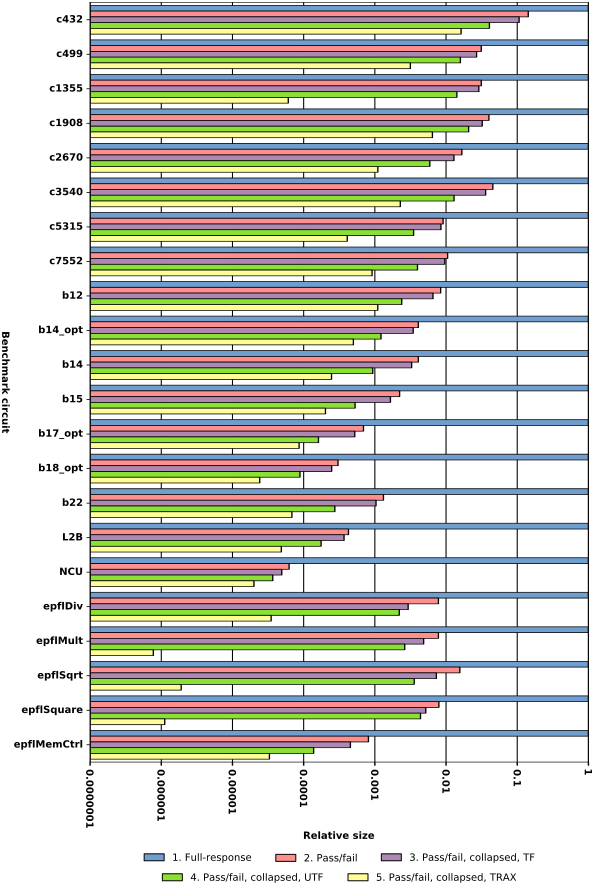
\includegraphics[width=\columnwidth]{fig_dictionary_histogram_vertical}
\caption{Comparison of fault-dictionary size for various compaction techniques.}
\label{fig:dict_histogram}
\end{figure}
%\vskip 0.5em%

Figure~\ref{fig:dict_histogram} shows the amount of dictionary size reduction resulting from the two compaction steps (pass/fail compaction, followed by equivalence and subsumption fault collapsing for the TRAX, UTF, and TF fault models) for several circuits.
%
This results in five fault dictionaries:
\begin{enumerate}
\item Full-response dictionary
\item Pass/fail dictionary
\item Pass/fail, collapsed, TF fault model dictionary
\item Pass/fail, collapsed, UTF fault model dictionary
\item Pass/fail, collapsed, TRAX fault model dictionary
\end{enumerate}
Both equivalence and subsumption fault collapsing are used for the TRAX and UTF dictionaries, however, because subsumption is not valid for the TF model, only equivalence fault collapsing is used for the TF dictionaries, resulting in very little additional compaction for TF.
%
While the use of hazard activation enables the TRAX fault model to subsume any glitch-caused failures in a circuit, the aggressive hazard activations result in the elimination of many faults by subsumption.
%
This produces a much smaller dictionary, but one with reduced diagnostic efficacy (evaluated in Chapter~\ref{chap:diag}).
%
Each design has five bars which show the relative size of each of the five dictionaries, on a logarithmic scale.
%
Each set is normalized to the size of the full-response dictionary.

On average, the dictionary size is reduced by 98.64\% for TF, reduced by 99.37\% for UTF, and reduced by 99.85\% for TRAX.
%
The maximum reduction for a UTF dictionary is for the NCU dictionary, which is compacted down to only 0.003683\% of the original size, a reduction by over 27,000x.
%
This reduces the NCU fault dictionary from 211 GB for the full-response dictionary to under 8 MB for the UTF compacted pass/fail dictionary.
%
For the TRAX dictionaries, the greatest compaction achieved is for the \verb+epflMult+ circuit, compacted down to only 0.00007734\% of the full-response size.
%
However, due to this incredible compaction, the dictionary does not retain much of its diagnostic ability.
%
The high compaction is due to this circuit having a few faults that fail very many of the applied tests.
%
Faults like this will eliminate many of the other faults in the same module via subsumption, leaving few faults (sometimes only one) remaining in each module.
%
Additionally, the EPFL circuits have very few input and output pins given the number of logic gates within each circuit, which reduces both controllability and observability for test generation.
%
Figure~\ref{fig:dict_gates_per_po} shows a plot of the gates per primary output for each analyzed circuit, showing that the EPFL circuits have many more gates per PO than the other benchmark circuits.
%
Further investigation of the often-failing faults is left as an area of future work.

%\vskip 0.5em%
\begin{figure}[htbp]
\centering
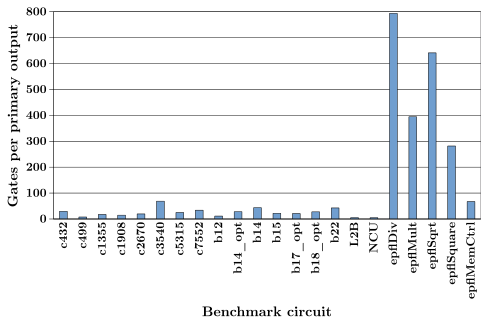
\includegraphics[width=0.8\columnwidth]{fig_dict_gates_per_po}
\caption{Comparison of the number of gates per primary output for each benchmark circuit.}
\label{fig:dict_gates_per_po}
\end{figure}
%\vskip 0.5em%

\subsection{Design Partition Sensitivity}
\label{sec:dict_exp_partitioning}

As previously mentioned, the non-ISCAS85 benchmarks lack any pre-existing module-level hierarchical and are partitioned into ten modules using graph clustering software.
%
A brief analysis is performed to determine the sensitivity of dictionary characteristics to the number of module partitions.
%
This analysis consists of repeatedly performing the following steps:
\begin{enumerate}
\item Use graph clustering to partition the circuit into $m$ modules.
\item Construct and compact the TRAX fault dictionary.
\item Evaluate diagnostic ability of resulting fault dictionary.
\end{enumerate}
These steps are performed for $m$ = 5 to 30, for both the L2B circuit (Figure~\ref{fig:dict_num_modules_clustering_l2b}) and the NCU circuit (Figure~\ref{fig:dict_num_modules_clustering_ncu}).
%
Details of the evaluation of diagnostic ability are provided in Section~\ref{sec:diag_exp_diag}, but in brief, the conventional metrics of Resolution and Accuracy are used here to evaluate a diagnosis result, including the use of \textit{Ideal Accurate} to describe a diagnosis result where the defective module is called-out as the most-likely responsible module.
%
As the number of module partitions increases from 5 to 30, there is a slight downward trend in the percentage of ideal accurate diagnosis results, and an upward trend in the size of the fault dictionary.
%
While it may appear counter-intuitive for the dictionary size to increase as the number of modules increase, which implies fewer faults per module, there is a logical explanation.
%
Dictionary compaction due to equivalence and subsumption is only applied to intra-module fault pairs, so more compaction is possible with larger modules and therefore more intra-module fault pairs.

%\vskip 0.5em%
\begin{figure}[htbp]
\centering
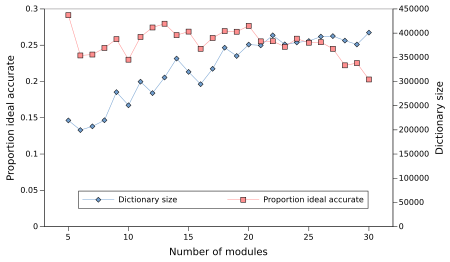
\includegraphics[width=0.9\columnwidth]{fig_dict_num_modules_clustering_l2b}
\caption{Experiments performed for L2B show that as the number of module partitions increase, there is a slight downward trend in ideal accurate diagnoses and a slight upward trend in dictionary size.}
\label{fig:dict_num_modules_clustering_l2b}
\end{figure}
%\vskip 0.5em%

%\vskip 0.5em%
\begin{figure}[htbp]
\centering
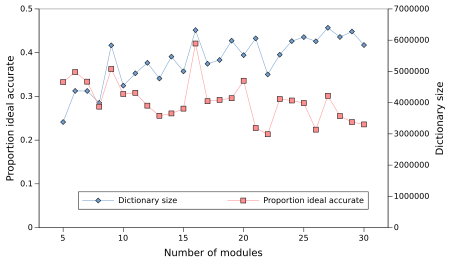
\includegraphics[width=0.9\columnwidth]{fig_dict_num_modules_clustering_ncu}
\caption{Experiments performed for NCU show that as the number of module partitions increase, there is a slight downward trend in ideal accurate diagnoses and a slight upward trend in dictionary size.}
\label{fig:dict_num_modules_clustering_ncu}
\end{figure}
%\vskip 0.5em%

While this may lead to the conclusion that a smaller number of modules is more desirable by these two metrics, this analysis does not include two important considerations.
%
When the number of modules is small, any detected defect will require the repair, replacement, or avoidance of a significant fraction of the core/uncore itself.
%
Furthermore, in the context of replacing modules, this reduces the ability of the core/uncore to recover from any future defects, as more of the available spare modules have been diagnosed as faulty and are unavailable for future use.
%
Taken to extremes, a core/uncore partitioned into a single module would have a zero-byte dictionary with perfect accuracy (every defect is located within the single ``module'' of the core/uncore), but the available recovery options are quite undesirable.
%
It is not very practical to wait to repair an entire core/uncore, replace the entire core/uncore, or try to avoid the core/uncore in its entirety.
%
At the other extreme, a core/uncore partitioned into dozens of modules would have a much larger fault dictionary with an associated reduced percentage of ideal accurate diagnosis results but would have more desirable recovery options available.
%
That is, repairing, replacing, or avoiding a small portion of a defective core/uncore is more appealing than doing the same for the entire core/uncore.
%
Additionally, when considering the replacement of defective modules, smaller and more numerous modules can handle more failures before running out of spare modules.
%
Consider the situation where a single spare is reserved for each module of a core/uncore.
%
If the core/uncore is partitioned into many modules, each can fail independently without reducing the overall functionality of the core/uncore.
%
If there are only a few modules, however, it is more likely that subsequent defects will lie within an already replaced module.

\section{Summary}
\label{sec:dict_summary}

To provide robustness against early-life and wear-out failures, the on-chip test and diagnosis environment localizes any detected failures using a hierarchical fault dictionary.
%
The relaxed diagnosis requirements (requiring defect localization only to the level of recovery) enable significant elimination of dictionary faults determined to be unnecessary for module-level diagnosis.
%
For intra-module faults with equivalent fault responses, all-but-one can be eliminated as redundant.
%
If the fault response of one fault subsumes the fault responses of any other intra-module faults, those subsumed faults can also be eliminated.
%
Dictionary compaction experiments show an average dictionary size reduction by 99.85\% for the TRAX fault dictionary.
%
For one of the largest analyzed circuits (NCU, part of the OpenSPARC T2 processor~\cite{sun11}) the dictionary is compacted down to only 0.00007734\% of the full-response size, reducing the dictionary size from 211 GB down to under 8 MB.
%
Additional analysis to determine the sensitivity of dictionary size and diagnostic ability to circuit partitioning determined a slight positive correlation between the number of partitions and the size of the dictionary, and a slight negative correlation between the number of partitions and the percentage of ideal accurate diagnosis results.
%
This analysis indicates that there is a trade-off to be made between partitioning a core/uncore into a fewer number of modules (with a smaller dictionary size and slightly-improved diagnosis outcome), and a larger number of modules (slightly-larger dictionary size but increased robustness in the face of multiple failing modules).
